% Options for packages loaded elsewhere
\PassOptionsToPackage{unicode}{hyperref}
\PassOptionsToPackage{hyphens}{url}
%
\documentclass[
]{book}
\title{A Minimal Book Example}
\author{John Doe}
\date{2022-09-14}

\usepackage{amsmath,amssymb}
\usepackage{lmodern}
\usepackage{iftex}
\ifPDFTeX
  \usepackage[T1]{fontenc}
  \usepackage[utf8]{inputenc}
  \usepackage{textcomp} % provide euro and other symbols
\else % if luatex or xetex
  \usepackage{unicode-math}
  \defaultfontfeatures{Scale=MatchLowercase}
  \defaultfontfeatures[\rmfamily]{Ligatures=TeX,Scale=1}
\fi
% Use upquote if available, for straight quotes in verbatim environments
\IfFileExists{upquote.sty}{\usepackage{upquote}}{}
\IfFileExists{microtype.sty}{% use microtype if available
  \usepackage[]{microtype}
  \UseMicrotypeSet[protrusion]{basicmath} % disable protrusion for tt fonts
}{}
\makeatletter
\@ifundefined{KOMAClassName}{% if non-KOMA class
  \IfFileExists{parskip.sty}{%
    \usepackage{parskip}
  }{% else
    \setlength{\parindent}{0pt}
    \setlength{\parskip}{6pt plus 2pt minus 1pt}}
}{% if KOMA class
  \KOMAoptions{parskip=half}}
\makeatother
\usepackage{xcolor}
\IfFileExists{xurl.sty}{\usepackage{xurl}}{} % add URL line breaks if available
\IfFileExists{bookmark.sty}{\usepackage{bookmark}}{\usepackage{hyperref}}
\hypersetup{
  pdftitle={A Minimal Book Example},
  pdfauthor={John Doe},
  hidelinks,
  pdfcreator={LaTeX via pandoc}}
\urlstyle{same} % disable monospaced font for URLs
\usepackage{color}
\usepackage{fancyvrb}
\newcommand{\VerbBar}{|}
\newcommand{\VERB}{\Verb[commandchars=\\\{\}]}
\DefineVerbatimEnvironment{Highlighting}{Verbatim}{commandchars=\\\{\}}
% Add ',fontsize=\small' for more characters per line
\usepackage{framed}
\definecolor{shadecolor}{RGB}{248,248,248}
\newenvironment{Shaded}{\begin{snugshade}}{\end{snugshade}}
\newcommand{\AlertTok}[1]{\textcolor[rgb]{0.94,0.16,0.16}{#1}}
\newcommand{\AnnotationTok}[1]{\textcolor[rgb]{0.56,0.35,0.01}{\textbf{\textit{#1}}}}
\newcommand{\AttributeTok}[1]{\textcolor[rgb]{0.77,0.63,0.00}{#1}}
\newcommand{\BaseNTok}[1]{\textcolor[rgb]{0.00,0.00,0.81}{#1}}
\newcommand{\BuiltInTok}[1]{#1}
\newcommand{\CharTok}[1]{\textcolor[rgb]{0.31,0.60,0.02}{#1}}
\newcommand{\CommentTok}[1]{\textcolor[rgb]{0.56,0.35,0.01}{\textit{#1}}}
\newcommand{\CommentVarTok}[1]{\textcolor[rgb]{0.56,0.35,0.01}{\textbf{\textit{#1}}}}
\newcommand{\ConstantTok}[1]{\textcolor[rgb]{0.00,0.00,0.00}{#1}}
\newcommand{\ControlFlowTok}[1]{\textcolor[rgb]{0.13,0.29,0.53}{\textbf{#1}}}
\newcommand{\DataTypeTok}[1]{\textcolor[rgb]{0.13,0.29,0.53}{#1}}
\newcommand{\DecValTok}[1]{\textcolor[rgb]{0.00,0.00,0.81}{#1}}
\newcommand{\DocumentationTok}[1]{\textcolor[rgb]{0.56,0.35,0.01}{\textbf{\textit{#1}}}}
\newcommand{\ErrorTok}[1]{\textcolor[rgb]{0.64,0.00,0.00}{\textbf{#1}}}
\newcommand{\ExtensionTok}[1]{#1}
\newcommand{\FloatTok}[1]{\textcolor[rgb]{0.00,0.00,0.81}{#1}}
\newcommand{\FunctionTok}[1]{\textcolor[rgb]{0.00,0.00,0.00}{#1}}
\newcommand{\ImportTok}[1]{#1}
\newcommand{\InformationTok}[1]{\textcolor[rgb]{0.56,0.35,0.01}{\textbf{\textit{#1}}}}
\newcommand{\KeywordTok}[1]{\textcolor[rgb]{0.13,0.29,0.53}{\textbf{#1}}}
\newcommand{\NormalTok}[1]{#1}
\newcommand{\OperatorTok}[1]{\textcolor[rgb]{0.81,0.36,0.00}{\textbf{#1}}}
\newcommand{\OtherTok}[1]{\textcolor[rgb]{0.56,0.35,0.01}{#1}}
\newcommand{\PreprocessorTok}[1]{\textcolor[rgb]{0.56,0.35,0.01}{\textit{#1}}}
\newcommand{\RegionMarkerTok}[1]{#1}
\newcommand{\SpecialCharTok}[1]{\textcolor[rgb]{0.00,0.00,0.00}{#1}}
\newcommand{\SpecialStringTok}[1]{\textcolor[rgb]{0.31,0.60,0.02}{#1}}
\newcommand{\StringTok}[1]{\textcolor[rgb]{0.31,0.60,0.02}{#1}}
\newcommand{\VariableTok}[1]{\textcolor[rgb]{0.00,0.00,0.00}{#1}}
\newcommand{\VerbatimStringTok}[1]{\textcolor[rgb]{0.31,0.60,0.02}{#1}}
\newcommand{\WarningTok}[1]{\textcolor[rgb]{0.56,0.35,0.01}{\textbf{\textit{#1}}}}
\usepackage{longtable,booktabs,array}
\usepackage{calc} % for calculating minipage widths
% Correct order of tables after \paragraph or \subparagraph
\usepackage{etoolbox}
\makeatletter
\patchcmd\longtable{\par}{\if@noskipsec\mbox{}\fi\par}{}{}
\makeatother
% Allow footnotes in longtable head/foot
\IfFileExists{footnotehyper.sty}{\usepackage{footnotehyper}}{\usepackage{footnote}}
\makesavenoteenv{longtable}
\usepackage{graphicx}
\makeatletter
\def\maxwidth{\ifdim\Gin@nat@width>\linewidth\linewidth\else\Gin@nat@width\fi}
\def\maxheight{\ifdim\Gin@nat@height>\textheight\textheight\else\Gin@nat@height\fi}
\makeatother
% Scale images if necessary, so that they will not overflow the page
% margins by default, and it is still possible to overwrite the defaults
% using explicit options in \includegraphics[width, height, ...]{}
\setkeys{Gin}{width=\maxwidth,height=\maxheight,keepaspectratio}
% Set default figure placement to htbp
\makeatletter
\def\fps@figure{htbp}
\makeatother
\setlength{\emergencystretch}{3em} % prevent overfull lines
\providecommand{\tightlist}{%
  \setlength{\itemsep}{0pt}\setlength{\parskip}{0pt}}
\setcounter{secnumdepth}{5}
\usepackage{booktabs}
\ifLuaTeX
  \usepackage{selnolig}  % disable illegal ligatures
\fi
\usepackage[]{natbib}
\bibliographystyle{plainnat}

\usepackage{amsthm}
\newtheorem{theorem}{Theorem}[chapter]
\newtheorem{lemma}{Lemma}[chapter]
\newtheorem{corollary}{Corollary}[chapter]
\newtheorem{proposition}{Proposition}[chapter]
\newtheorem{conjecture}{Conjecture}[chapter]
\theoremstyle{definition}
\newtheorem{definition}{Definition}[chapter]
\theoremstyle{definition}
\newtheorem{example}{Example}[chapter]
\theoremstyle{definition}
\newtheorem{exercise}{Exercise}[chapter]
\theoremstyle{definition}
\newtheorem{hypothesis}{Hypothesis}[chapter]
\theoremstyle{remark}
\newtheorem*{remark}{Remark}
\newtheorem*{solution}{Solution}
\begin{document}
\maketitle

{
\setcounter{tocdepth}{1}
\tableofcontents
}
\hypertarget{about}{%
\chapter{About}\label{about}}

This is a \emph{sample} book written in \textbf{Markdown}. You can use anything that Pandoc's Markdown supports; for example, a math equation \(a^2 + b^2 = c^2\).

\hypertarget{section}{%
\chapter{2022}\label{section}}

\hypertarget{boot-camp-for-beginners}{%
\section{Boot Camp for Beginners}\label{boot-camp-for-beginners}}

\hypertarget{what-is-causal-inference}{%
\subsection{What is Causal Inference?}\label{what-is-causal-inference}}

\hypertarget{potential-outcome-framework-regression-and-matching}{%
\subsection{Potential Outcome Framework, Regression, and Matching}\label{potential-outcome-framework-regression-and-matching}}

\begin{itemize}
\tightlist
\item
  In some special cases, conditioning may not work as it causes other backdoor paths to open. In this case, weighting methods can be used.
\end{itemize}

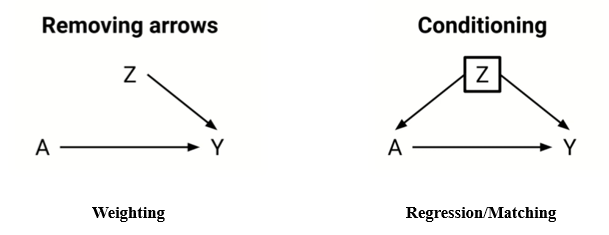
\includegraphics{figures/01.png}

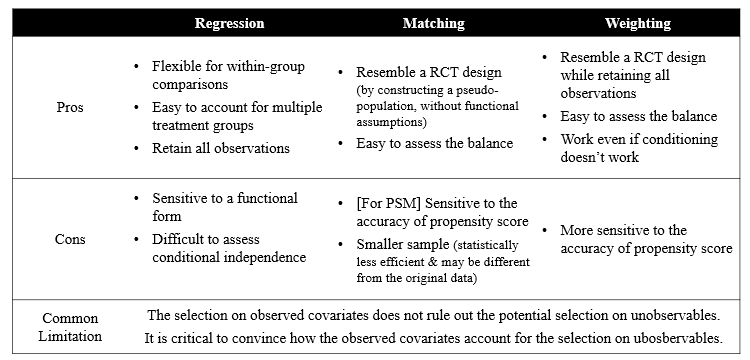
\includegraphics{figures/02.png}

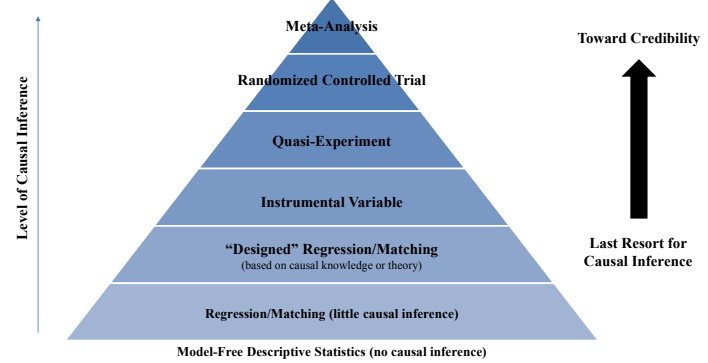
\includegraphics{figures/03.png}

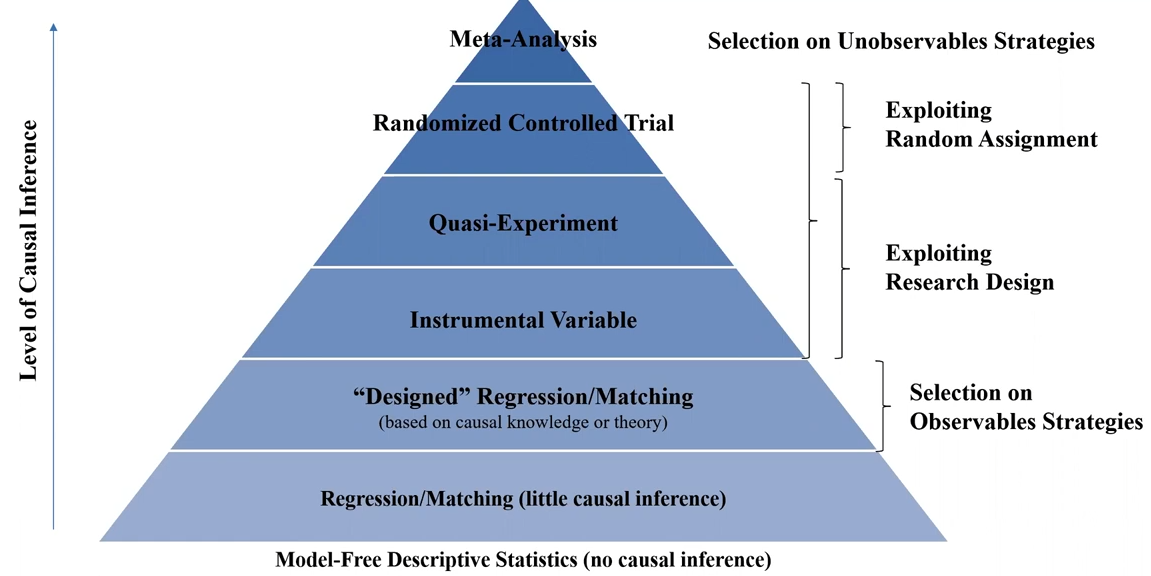
\includegraphics{figures/22.png}

\begin{itemize}
\tightlist
\item
  Selection on observables does not guarantee the balance of unobserved covariates.
\item
  Selection on observables strategies should be considered the last resort for causal inference, as it is quite challenging to account for unobserved variables by using only observed variables.
\item
  Control variables, matching, or weighting are still helpful in making randomized controlled trials or quasi-experiments more rigorous. It is more common to utilize control variables, matching, or weighting in tandem with other experimental methods, rather than in isolation.
\item
  \emph{Ceteris Paribus} in the presence of control variables, matching, or weighting

  \begin{itemize}
  \tightlist
  \item
    The control group should be comparable to the treatment group in all aspects, except control variables, but the fact that they are treated.
  \end{itemize}
\end{itemize}

\hypertarget{quasi-experiments}{%
\subsection{Quasi-Experiments}\label{quasi-experiments}}

\begin{itemize}
\tightlist
\item
  Quasi-experiment = Research Designs without random assignment

  \begin{itemize}
  \tightlist
  \item
    The only difference between RCT and quasi-experiment lies at the treatment assignment mechanism.
  \end{itemize}
\item
  Quasi-experiment is a research design where a control group is comparable to the treatment, not randomly assigned, except the fact that they didn't receive the treatment.

  \begin{itemize}
  \tightlist
  \item
    Key Identification Assumption

    \begin{itemize}
    \tightlist
    \item
      Is the treatment assignment without random assignment as good as random?
    \item
      How similar is the control group to the treatment group is the absence of the treatment?
    \end{itemize}
  \end{itemize}
\item
  Causation is defined as the difference in potential outcomes after the treatment.

  \begin{itemize}
  \tightlist
  \item
    Causal effect = (Actual outcome for treated if treated) -- (Potential outcome for treated if not treated) = \emph{Counterfactual}
  \end{itemize}
\end{itemize}

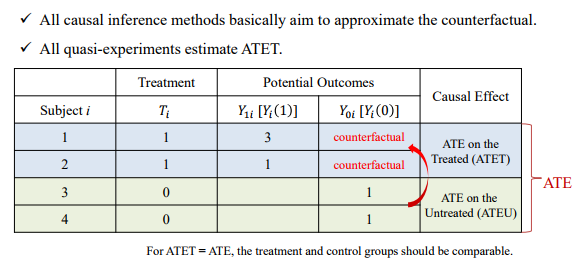
\includegraphics{figures/23.png}

\begin{itemize}
\item
  Data Structure from the Perspective of Counterfactual

  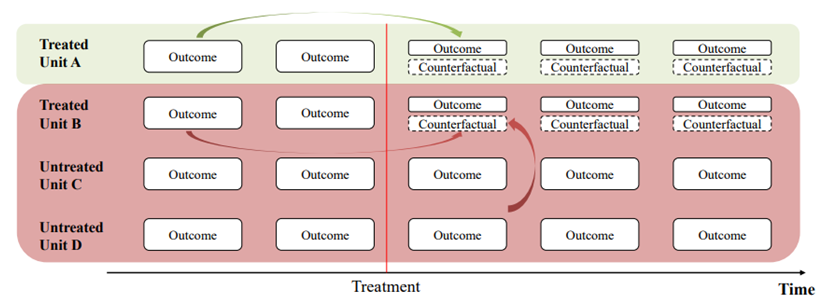
\includegraphics{figures/24.png}
\item
  What's Your Research Design and Data Structure?

  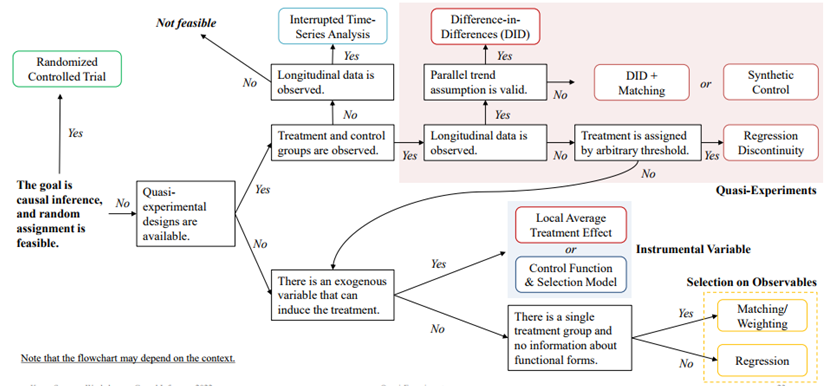
\includegraphics{figures/25.png}
\item
  Difference-in-Differences

  \begin{itemize}
  \tightlist
  \item
    With panel data, DID approximates the counterfactual using its own prior and time trends of the control group.
  \item
    For DID analysis, the parallel trend assumption (in the absence of treatment) must be hold.

    \begin{itemize}
    \tightlist
    \item
      Basically, the parallel trend assumption is not verifiable, and what we can show is parallel pretrends.
    \item
      Matching methods might help to achieve the parallel trend assumption.
    \end{itemize}
  \end{itemize}
\end{itemize}

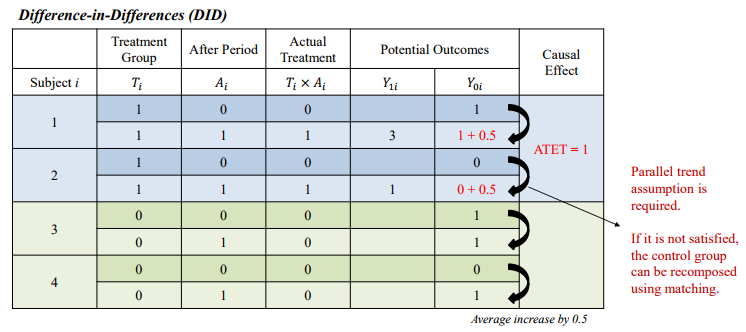
\includegraphics{figures/26.png}

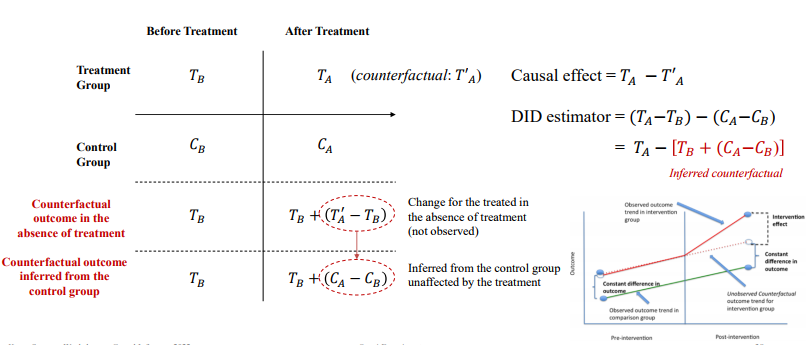
\includegraphics{figures/31.png}

\begin{itemize}
\tightlist
\item
  Synthetic Control

  \begin{itemize}
  \tightlist
  \item
    With panel data, SC approximates the counterfactual using a combination of the control group.
  \item
    Synthetic control method is in line with difference-in-differences in that they approximate the counterfactual using untreated units in the control group.
  \end{itemize}
\end{itemize}

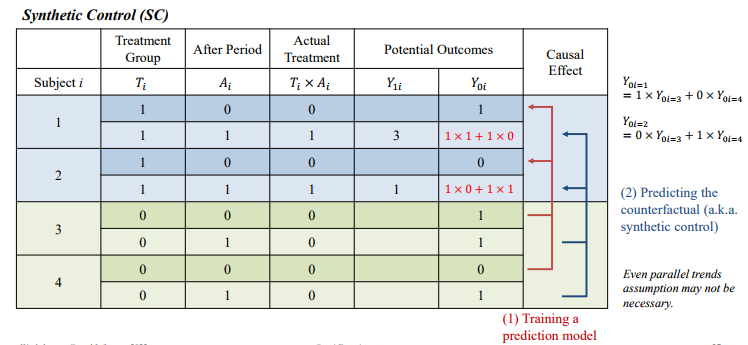
\includegraphics{figures/27.png}

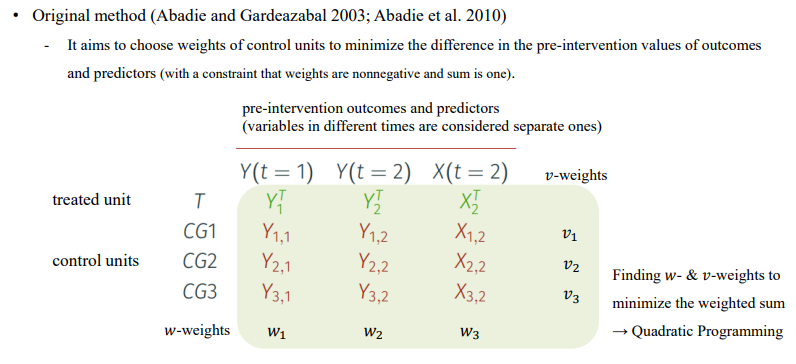
\includegraphics{figures/32.png}

\begin{itemize}
\item
  Synthetic Control vs.~Difference-in-Differences

  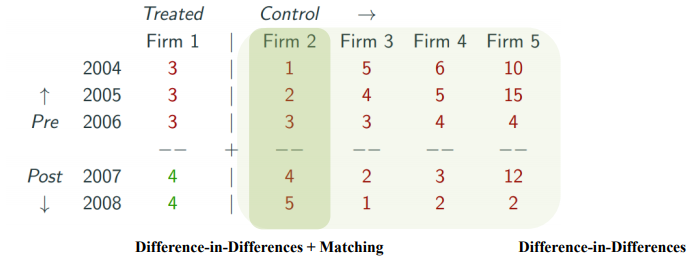
\includegraphics{figures/28.png}

  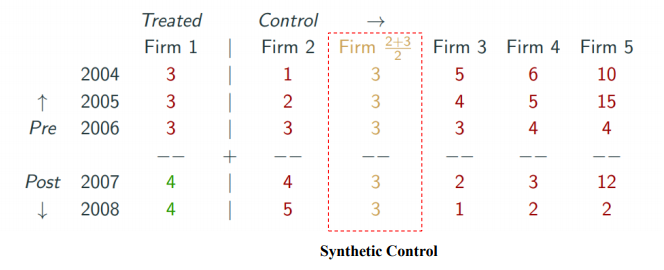
\includegraphics{figures/29.png}
\item
  Interrupted Time-Series Analysis

  \begin{itemize}
  \tightlist
  \item
    With pure time-series data, interrupted time-series analysis approximates the counterfactual using its own prior and time trends.
  \item
    In the case of no control group, time-series forecasting models can be used to predict the counterfactual.
  \item
    See \textbf{CausalImpact} R package
  \end{itemize}
\end{itemize}

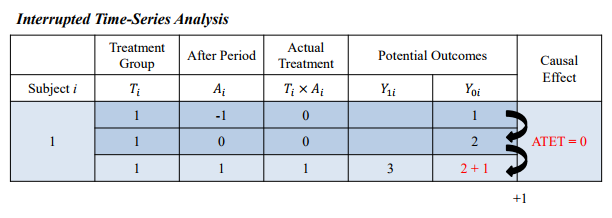
\includegraphics{figures/30.png}

\hypertarget{instrumental-variable-and-regression-discontinuity}{%
\subsection{Instrumental Variable and Regression Discontinuity}\label{instrumental-variable-and-regression-discontinuity}}

\begin{itemize}
\item
  To interpret the regression in a causal manner, the treatment variable should not be correlated with the error term capturing all unobserved factors that could influence the outcome variable.
\item
  Instrumental variable (IV) is an instrument to separate the exogenous portion of the treatment variable from the endogenous portion (selection bias).

  \begin{itemize}
  \item
    \begin{enumerate}
    \def\labelenumi{(\arabic{enumi})}
    \tightlist
    \item
      The IVs should be correlated with the endogenous treatment variable (relevance).
    \end{enumerate}
  \item
    \begin{enumerate}
    \def\labelenumi{(\arabic{enumi})}
    \setcounter{enumi}{1}
    \tightlist
    \item
      The IVs should not be correlated with the error term in the explanatory equation.
    \end{enumerate}

    \begin{itemize}
    \tightlist
    \item
      Exclusion restriction: The IVs do not affect the outcome except through the treatment variable.
    \item
      Exogeneity of IV: The IVs do not share any confounders with the outcome.
    \end{itemize}
  \end{itemize}
\end{itemize}

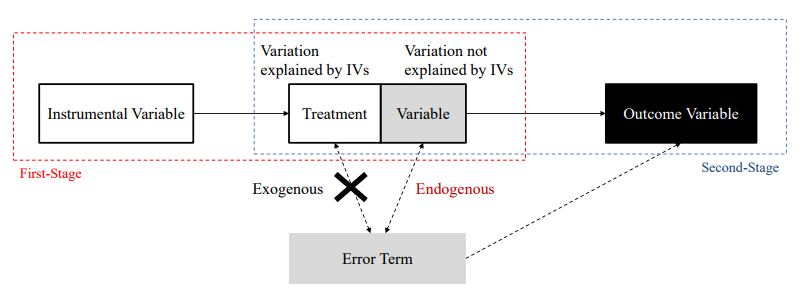
\includegraphics{figures/33.png}

\begin{itemize}
\tightlist
\item
  Regression Discontinuity (RD)

  \begin{itemize}
  \tightlist
  \item
    Regression discontinuity is to identify the local discontinuous jump on a running (assignment) variable.
  \item
    The estimation of treatment effect in RD depends on extrapolation based on a running variable (dashed line).
  \end{itemize}
\end{itemize}

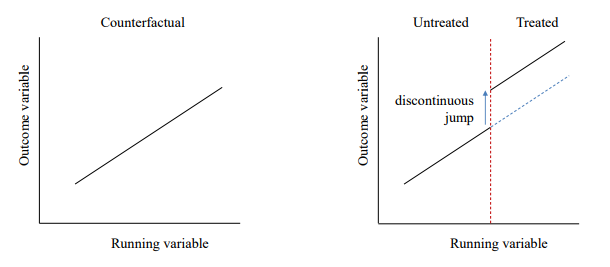
\includegraphics{figures/34.png}

\hypertarget{causal-graph-and-structural-causal-model}{%
\subsection{Causal Graph and Structural Causal Model}\label{causal-graph-and-structural-causal-model}}

\begin{itemize}
\tightlist
\item
  Directed Acyclic Graph (DAG)

  \begin{itemize}
  \tightlist
  \item
    Graph: A structure made from nodes and edges
  \item
    Directed: Direction represents a causal relationship between nodes
  \item
    Acyclic: No directed cycles
  \end{itemize}
\end{itemize}

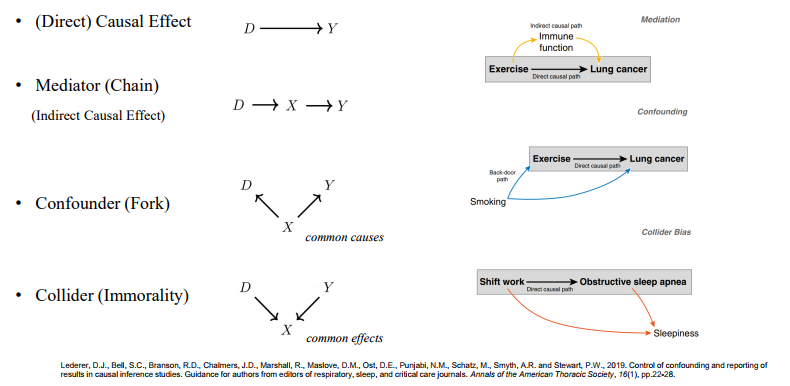
\includegraphics{figures/35.png}

\begin{itemize}
\tightlist
\item
  Association in Causal Graph
\end{itemize}

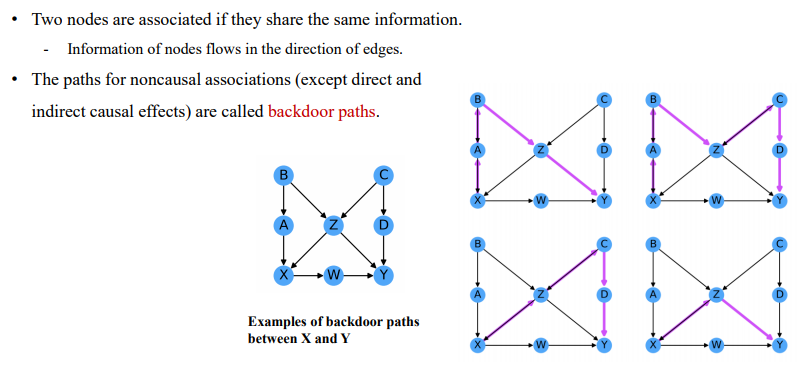
\includegraphics{figures/36.png}

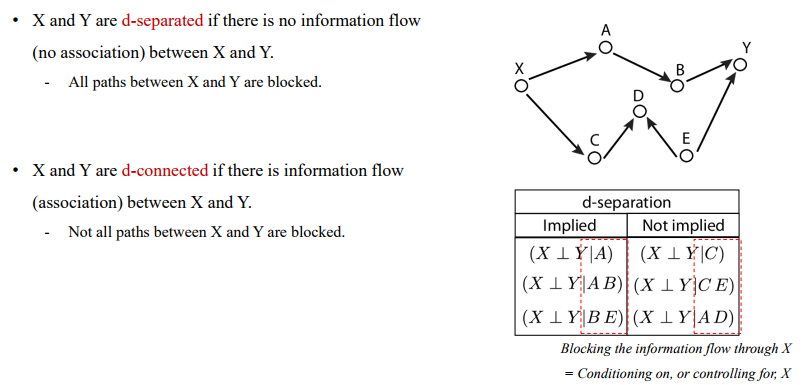
\includegraphics{figures/37.png}

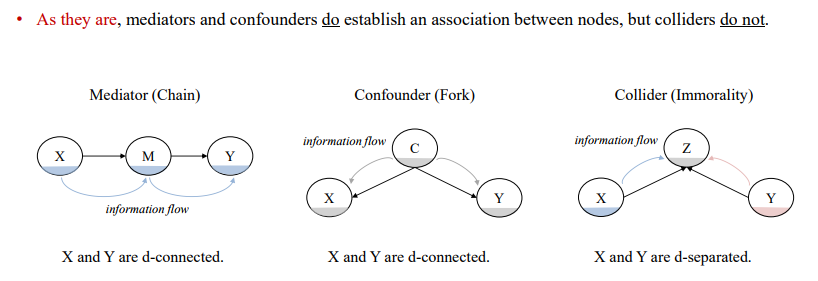
\includegraphics{figures/38.png}

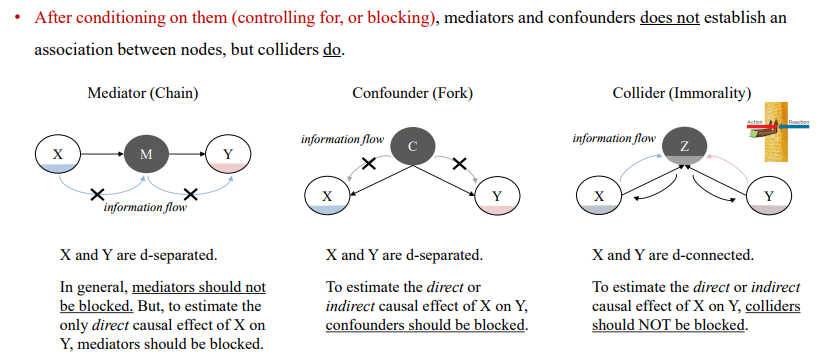
\includegraphics{figures/39.png}

\begin{itemize}
\tightlist
\item
  Applications of Causal Graph for Design-Based Approach

  \begin{itemize}
  \item
    \begin{enumerate}
    \def\labelenumi{(\arabic{enumi})}
    \tightlist
    \item
      Structure-Based Research Design
    \end{enumerate}
  \end{itemize}
\end{itemize}

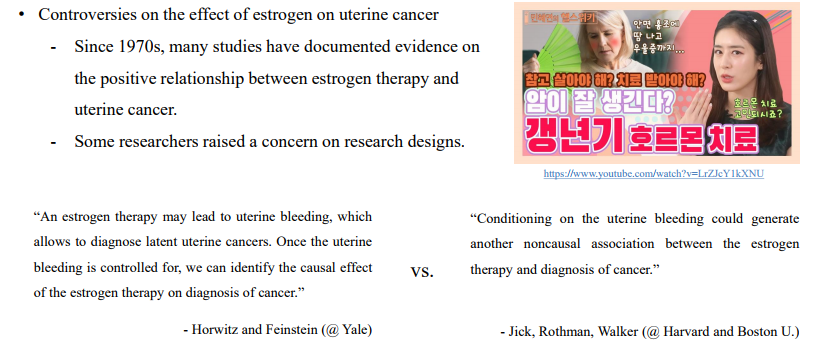
\includegraphics{figures/40.png}

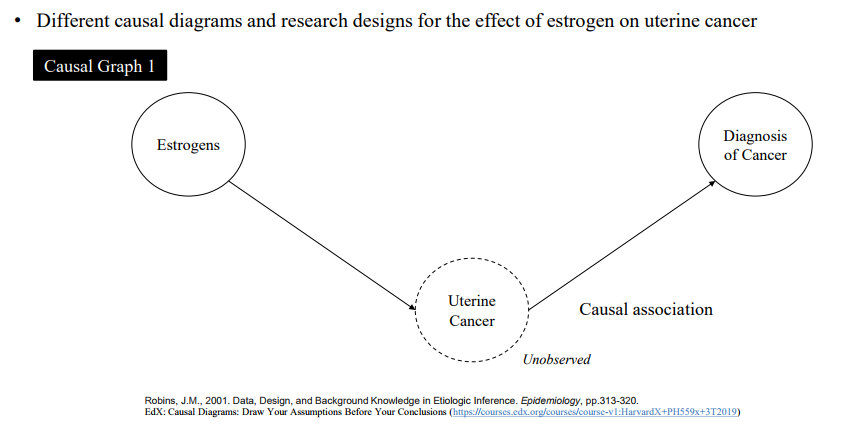
\includegraphics{figures/41.png}

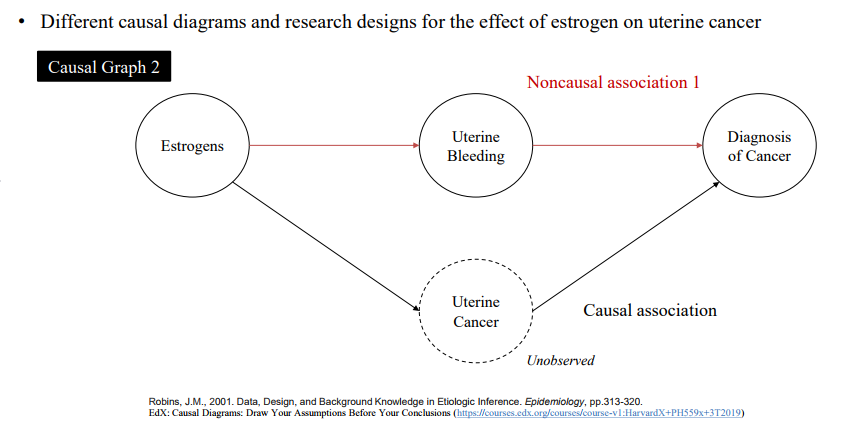
\includegraphics{figures/42.png}

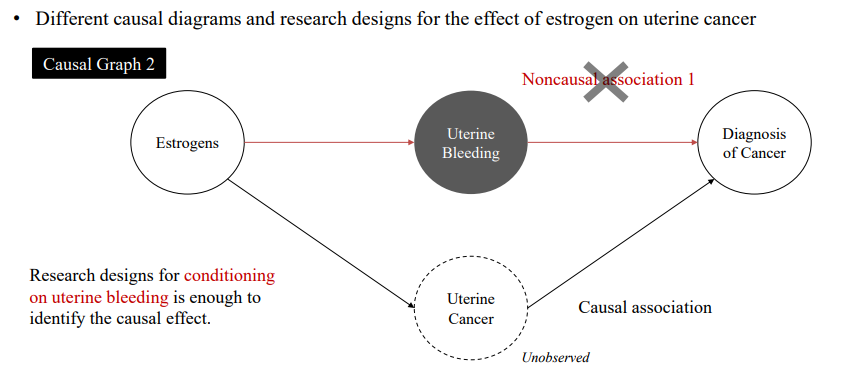
\includegraphics{figures/43.png}

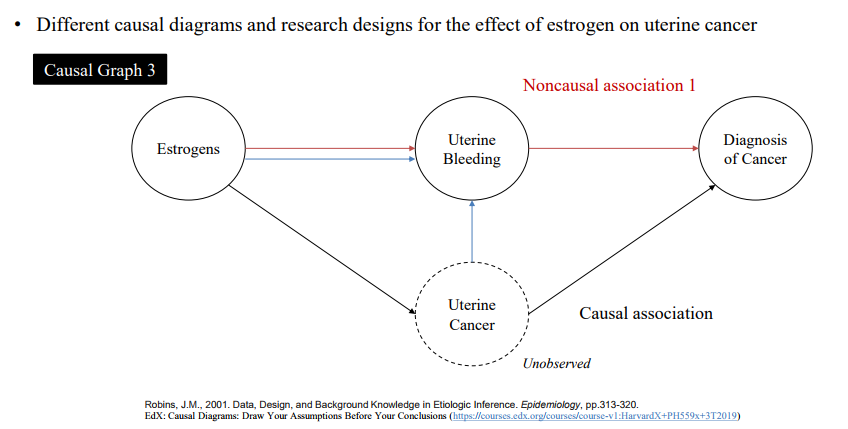
\includegraphics{figures/44.png}

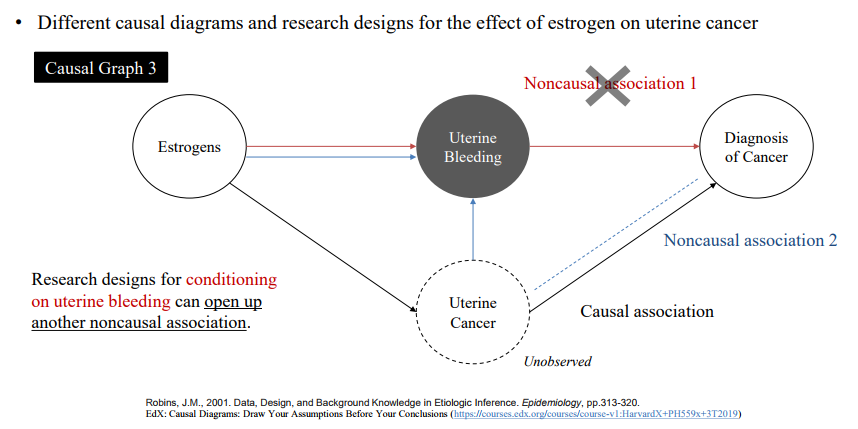
\includegraphics{figures/45.png}

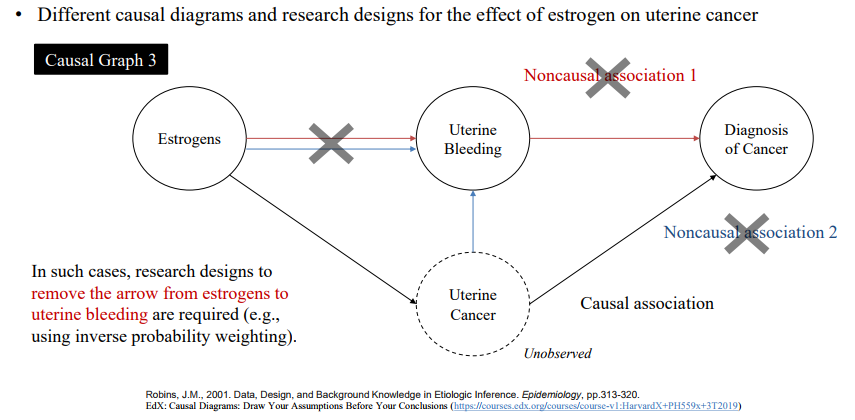
\includegraphics{figures/46.png}

\begin{itemize}
\item
  \begin{enumerate}
  \def\labelenumi{(\arabic{enumi})}
  \setcounter{enumi}{1}
  \tightlist
  \item
    Design of Control Variables / Conditioning Strategies
  \end{enumerate}
\end{itemize}

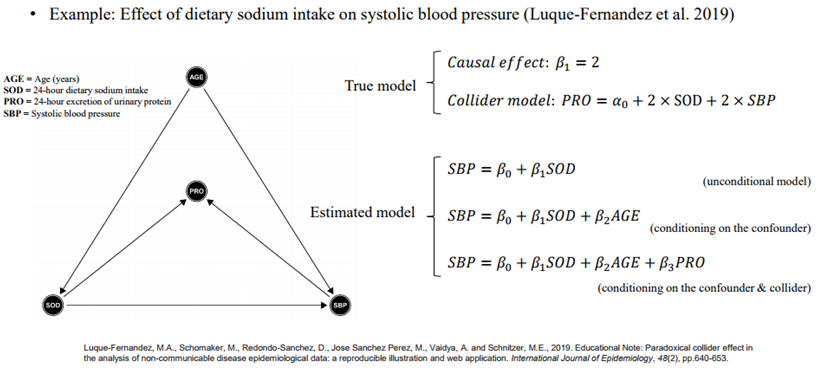
\includegraphics{figures/47.png}

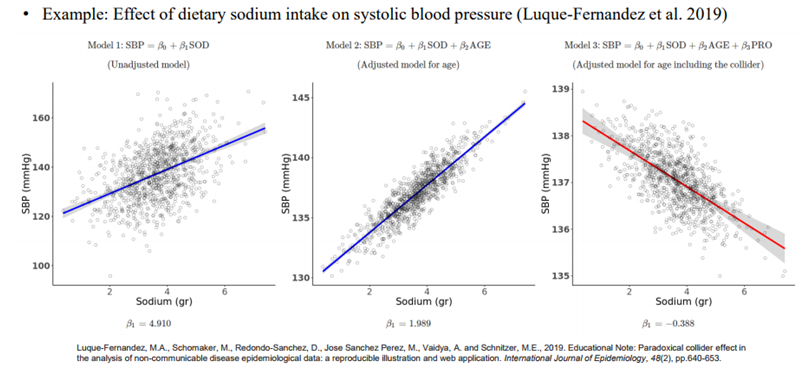
\includegraphics{figures/48.png}

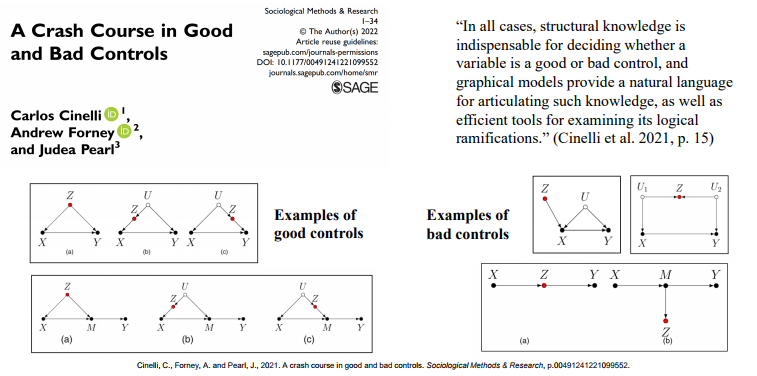
\includegraphics{figures/49.png}

\begin{itemize}
\item
  \begin{enumerate}
  \def\labelenumi{(\arabic{enumi})}
  \setcounter{enumi}{2}
  \tightlist
  \item
    Communicating Identification Assumptions
  \end{enumerate}
\item
  \begin{enumerate}
  \def\labelenumi{(\arabic{enumi})}
  \setcounter{enumi}{3}
  \tightlist
  \item
    Transportability: From RCTs to Observational Studies
  \end{enumerate}
\item
  Structural Causal Model = Probabilistic Causal Mechanisms
\end{itemize}

\hypertarget{health-informatics-marketing}{%
\section{Health Informatics \& Marketing}\label{health-informatics-marketing}}

\hypertarget{heterogeneous-treatment-effect-estimation-using-machine-learning---application-to-healthcare-data}{%
\subsection{Heterogeneous Treatment Effect Estimation Using Machine Learning - Application to Healthcare Data}\label{heterogeneous-treatment-effect-estimation-using-machine-learning---application-to-healthcare-data}}

\begin{itemize}
\tightlist
\item
  Developing a drug: ``from the new'' vs.~``recycling''
\end{itemize}

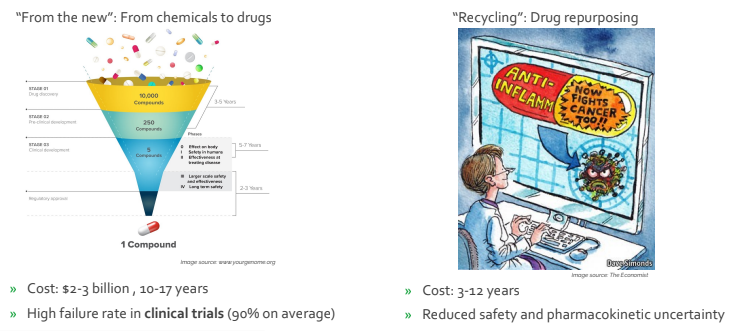
\includegraphics{figures/04.png}

\begin{itemize}
\tightlist
\item
  What is Randomized clinicaltrials (RCTs)?

  \begin{itemize}
  \tightlist
  \item
    ``Gold standard'' for testing treatments in people
  \item
    Test the treatment's effectiveness by making a fair
    comparison
  \item
    Participants are divided by chance into separate groups

    \begin{itemize}
    \tightlist
    \item
      Treatment(s) group: receive a new treatment
    \item
      Placebo group: receive standard treatment
    \end{itemize}
  \item
    Expensive, high failure rate, sometimes not safe

    \begin{itemize}
    \tightlist
    \item
      Emulate the RCTs using real-world observation!
    \end{itemize}
  \end{itemize}
\item
  Emulate RCTs using real-world observation (For existing drugs)
\end{itemize}

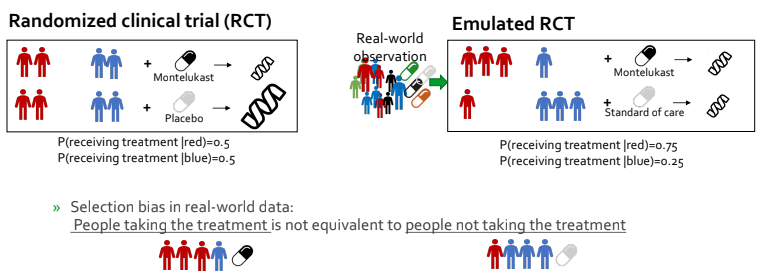
\includegraphics{figures/05.png}

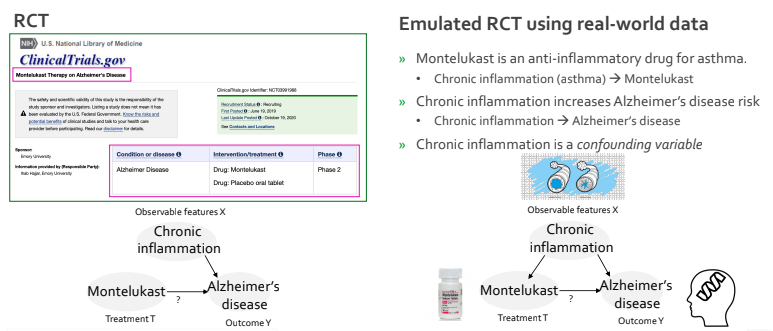
\includegraphics{figures/06.png}

\begin{itemize}
\tightlist
\item
  Challenge 1: Selection bias

  \begin{itemize}
  \tightlist
  \item
    Potential outcomes model
  \item
    Propensity score
  \item
    Average treatment effect
  \end{itemize}
\end{itemize}

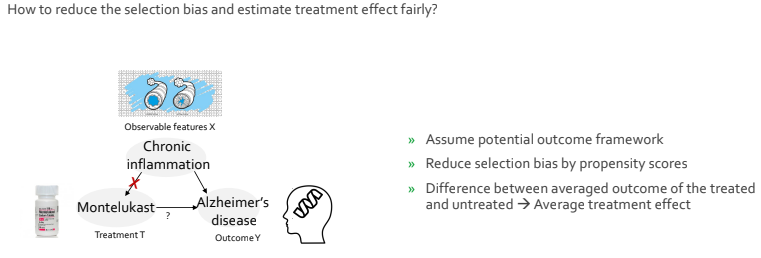
\includegraphics{figures/07.png}

\strut \\

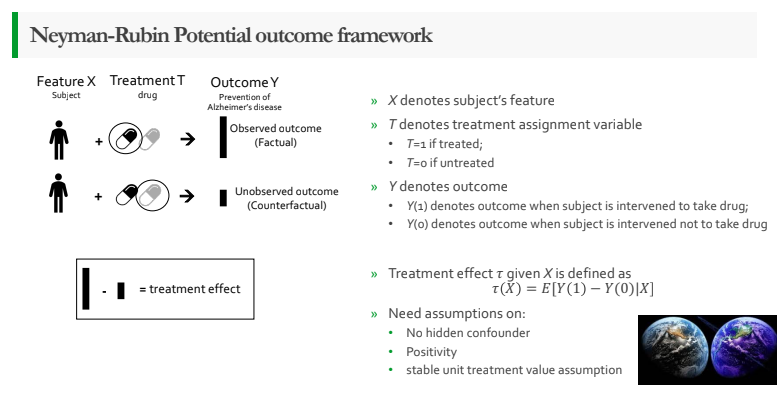
\includegraphics{figures/08.png}

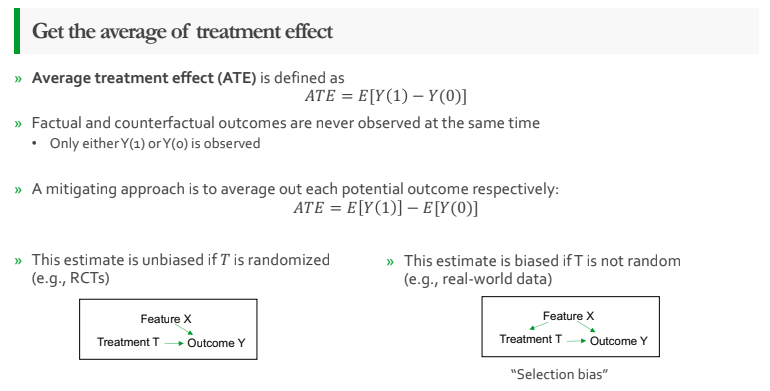
\includegraphics{figures/09.png}

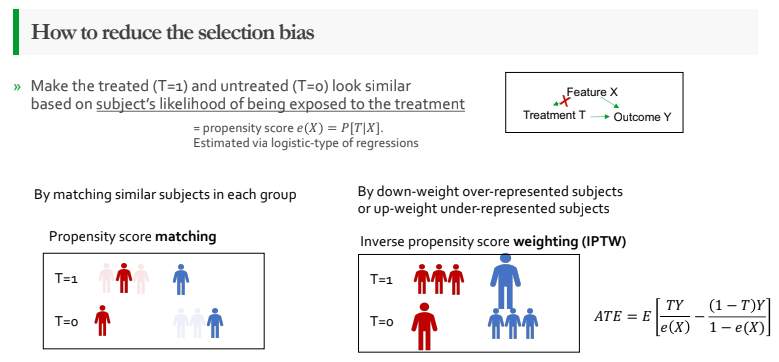
\includegraphics{figures/10.png}

\begin{itemize}
\tightlist
\item
  Challenge 2: Heterogeneity in treatment effect

  \begin{itemize}
  \tightlist
  \item
    Double machine learning
  \item
    Meta learners
  \item
    Balanced representation learning
  \end{itemize}
\end{itemize}

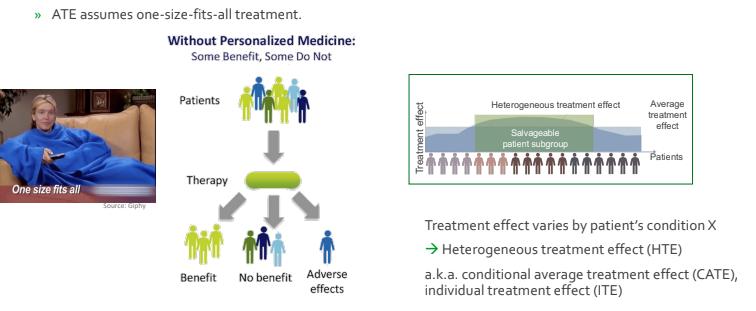
\includegraphics{figures/11.png}

\begin{itemize}
\tightlist
\item
  How to estimate the heterogeneous treatment effect?

  \begin{itemize}
  \tightlist
  \item
    High-level steps

    \begin{itemize}
    \tightlist
    \item
      Learn ``nuisance'' or ``context'' around feature X via regression
    \item
      Estimate the HTE by learning coefficient in semi-parametric structural equation model or imputing counterfactual outcomes
    \item
      Optionally weight the outcome estimate by propensity score
    \end{itemize}
  \item
    Methods: double machine learning, meta learners, balanced representation learning, etc.
  \end{itemize}
\end{itemize}

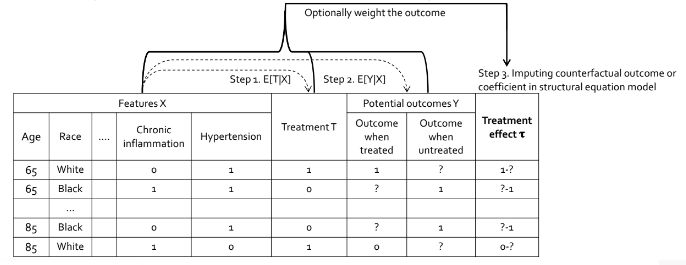
\includegraphics{figures/12.png}

\begin{itemize}
\tightlist
\item
  Double Machine Learning (Chernozhukov 2016)
\end{itemize}

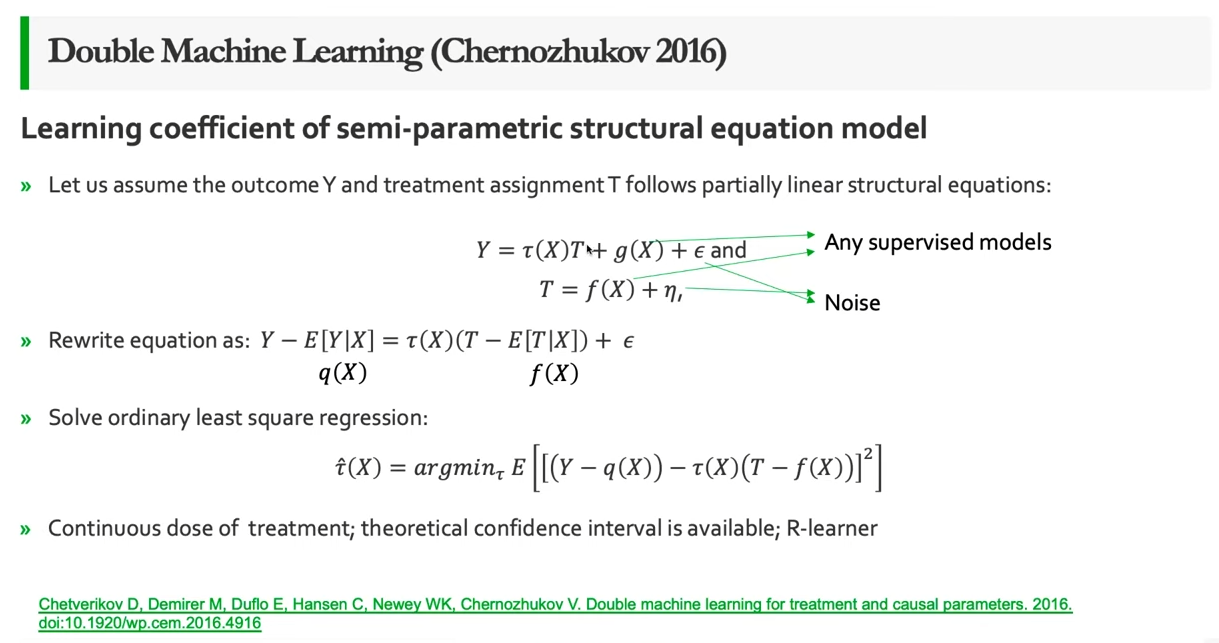
\includegraphics{figures/13.png}

\begin{itemize}
\tightlist
\item
  Meta learners
\end{itemize}

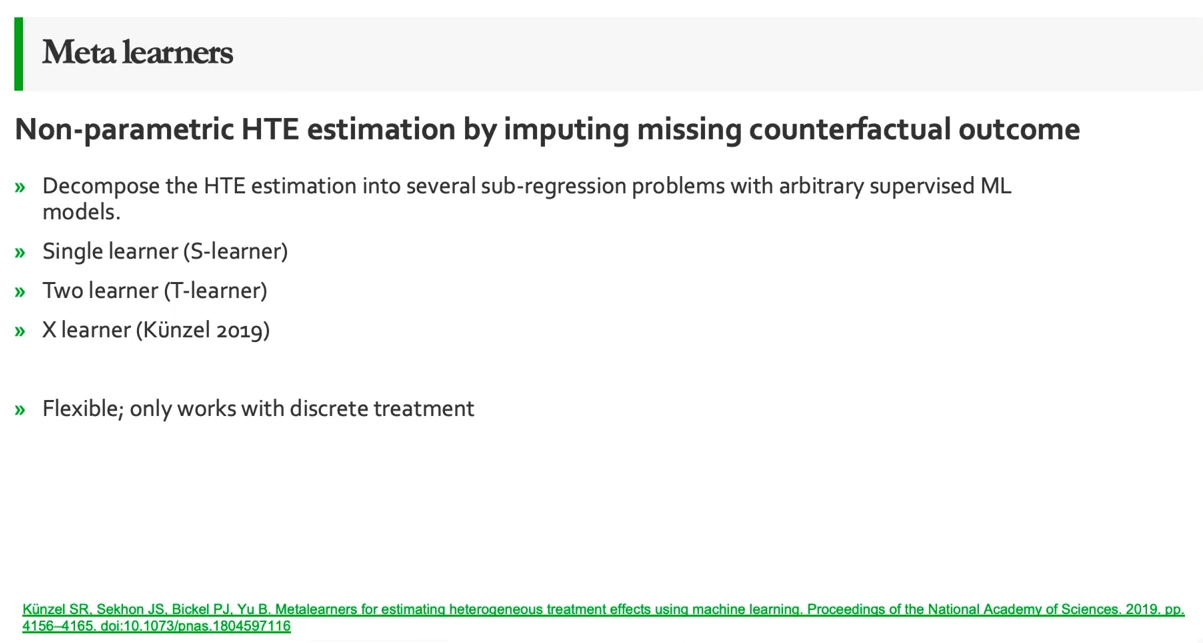
\includegraphics{figures/14.png}

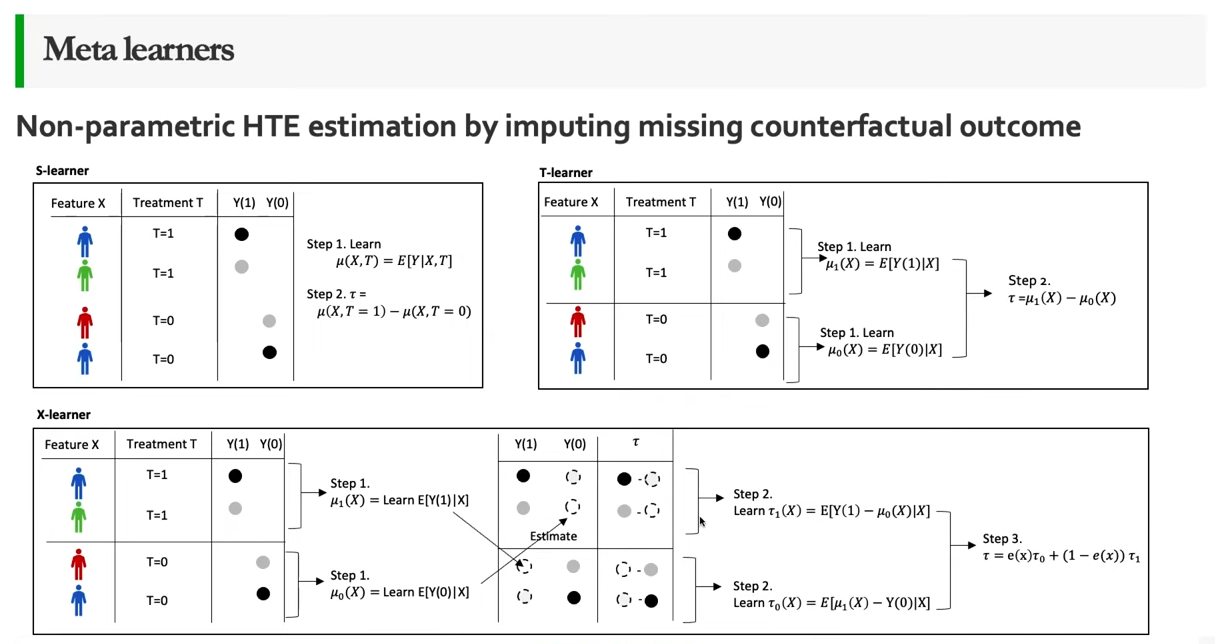
\includegraphics{figures/15.png}

\begin{itemize}
\tightlist
\item
  Balanced representation learning
\end{itemize}

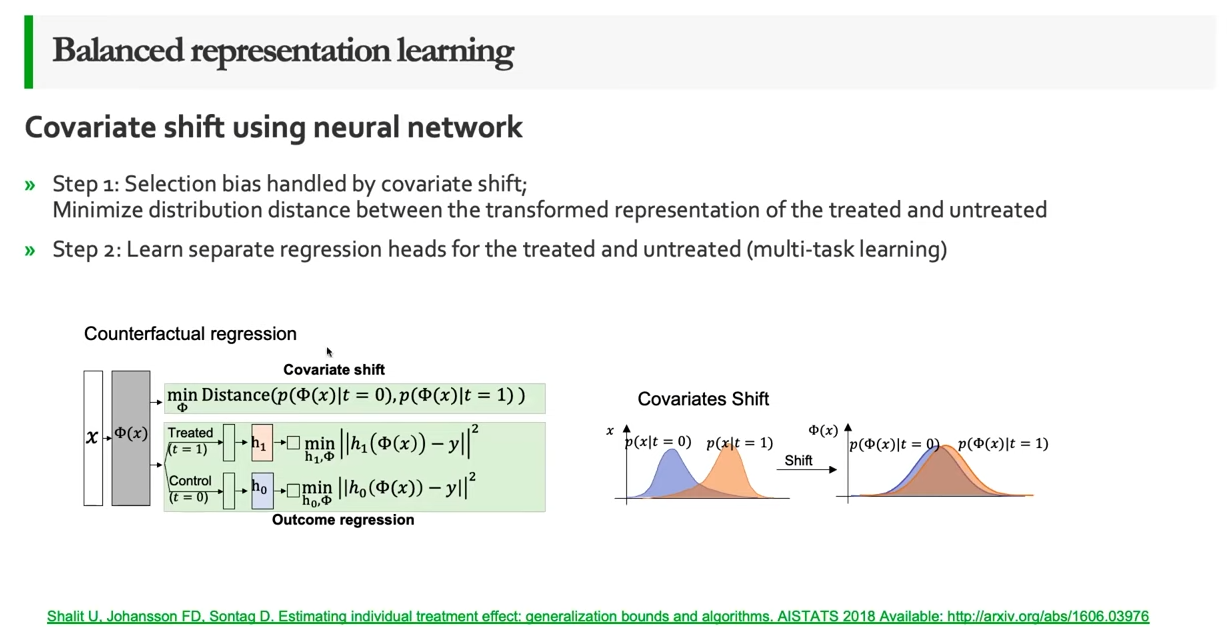
\includegraphics{figures/16.png}

\begin{itemize}
\tightlist
\item
  Methodology comparison
\end{itemize}

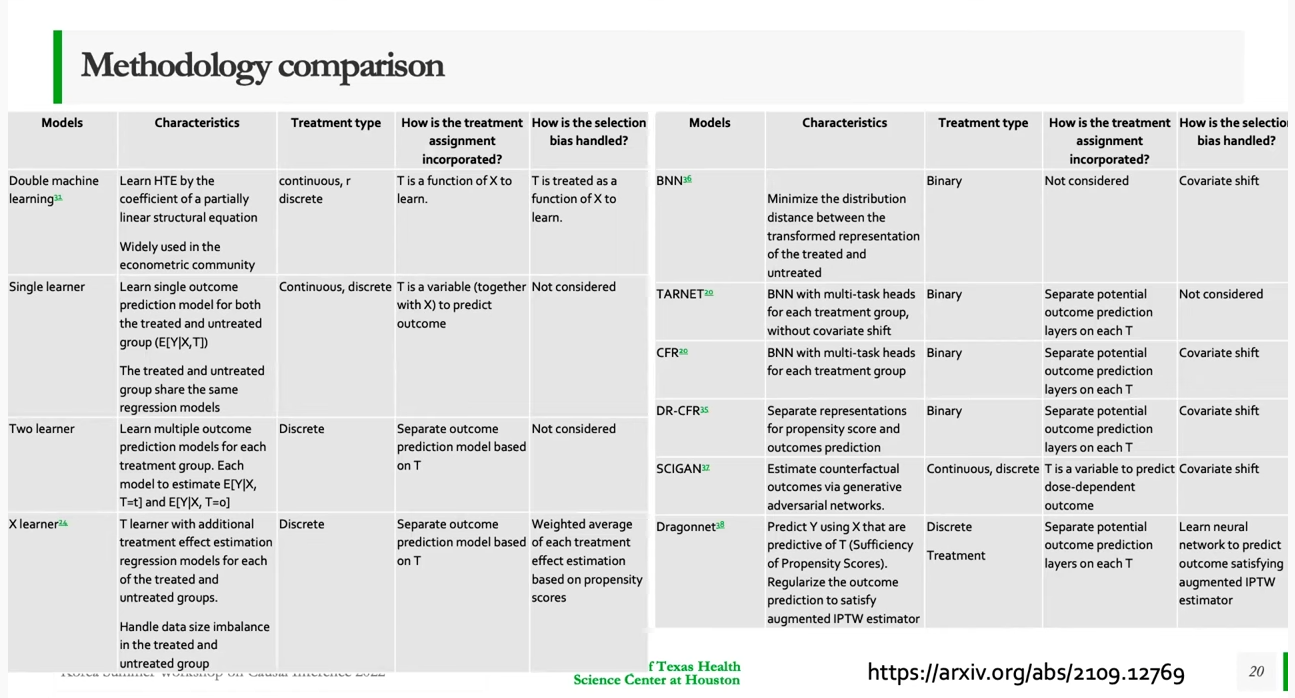
\includegraphics{figures/17.png}

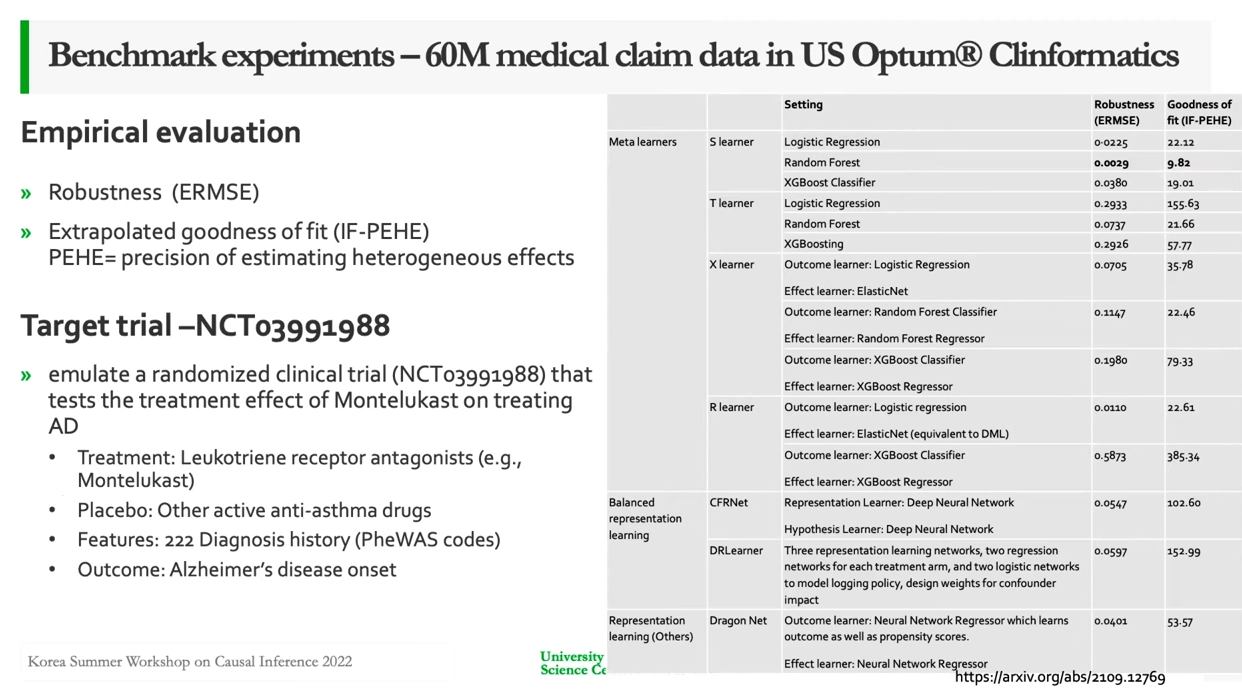
\includegraphics{figures/18.png}

\strut \\

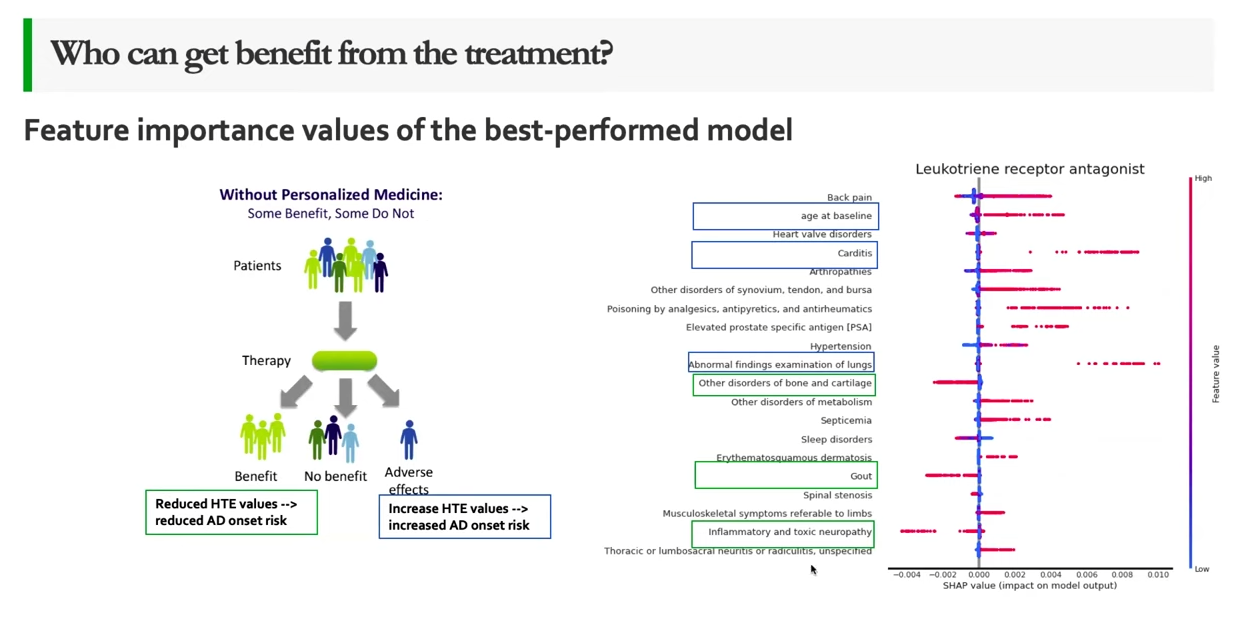
\includegraphics{figures/19.png}

\strut \\

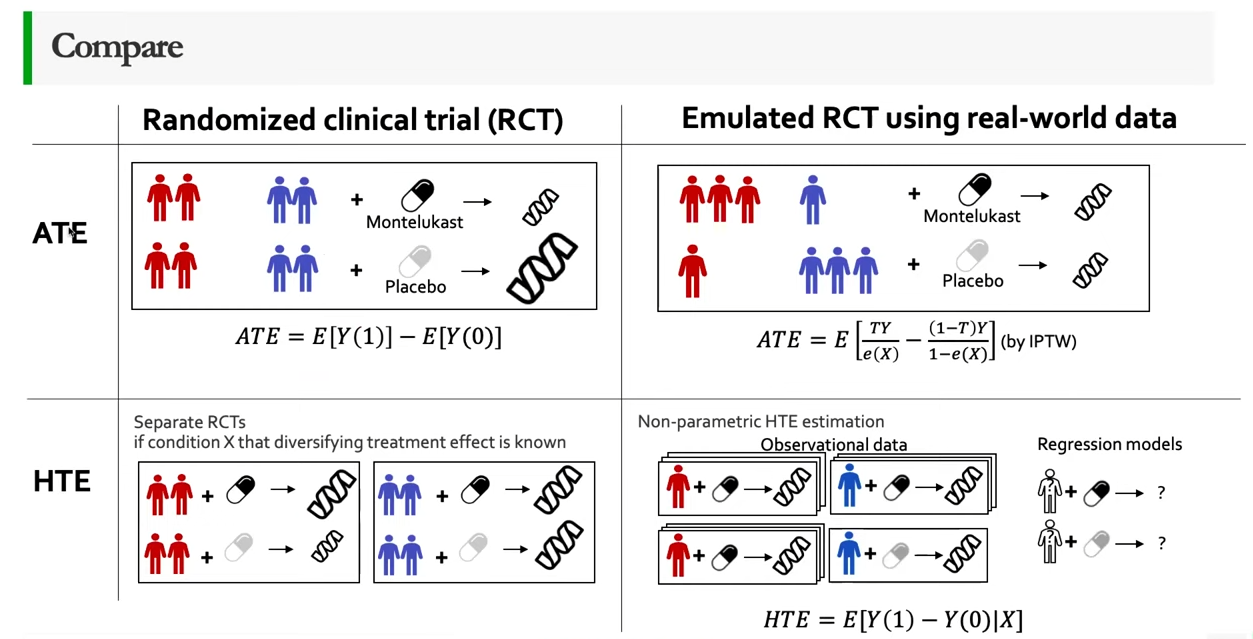
\includegraphics{figures/20.png}

\strut \\

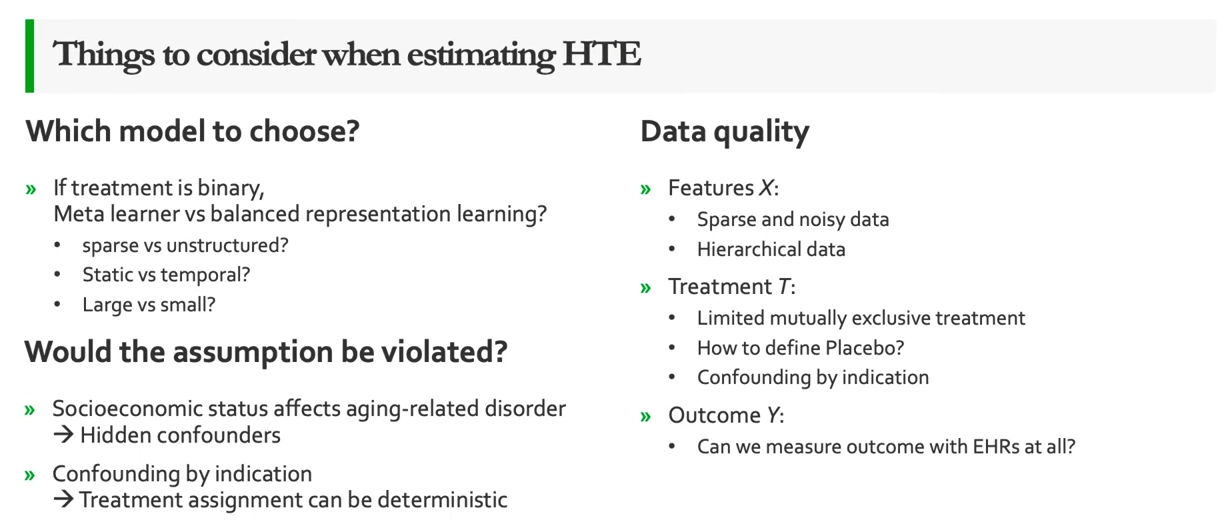
\includegraphics{figures/21.png}

\hypertarget{korea-summer-session-on-causal-inference-2021}{%
\chapter{Korea Summer Session on Causal Inference 2021}\label{korea-summer-session-on-causal-inference-2021}}

\hypertarget{session-introduction}{%
\section{Session Introduction}\label{session-introduction}}

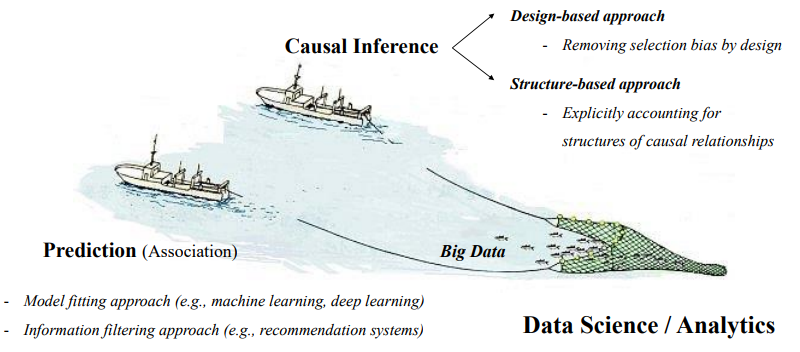
\includegraphics{figures/50.png}

\hypertarget{module-1.-research-design-for-causal-inference}{%
\section{Module 1. Research Design for Causal Inference}\label{module-1.-research-design-for-causal-inference}}

\hypertarget{session-1.-potential-outcomes-framework-causal-mindset}{%
\subsection{Session 1. Potential Outcomes Framework: Causal Mindset}\label{session-1.-potential-outcomes-framework-causal-mindset}}

\begin{itemize}
\tightlist
\item
  Potential Outcomes Framework

  \begin{itemize}
  \tightlist
  \item
    Causation is defined as the difference in potential outcomes after the treatment.
  \item
    Causal effect of the treatment = (Actual outcome for treated if treated) -- (Potential outcome for treated if not treated)

    \begin{itemize}
    \tightlist
    \item
      Average Treatment Effect (ATE) on the Treated (ATT)
    \end{itemize}
  \item
    By definition, potential outcomes are not always observable. The fundamental challenge in causal inference is that we do not observe both potential outcomes; we only observe one.

    \begin{itemize}
    \tightlist
    \item
      But, in reality, we can only observe = (Actual outcome for treated if treated) -- (Actual outcome for untreated if not treated).
    \end{itemize}
  \end{itemize}
\item
  Selection Bias

  \begin{itemize}
  \tightlist
  \item
    In reality, any treatments are not assigned randomly. Individuals select the treatment (but we don't know why).
  \item
    As a result, the treatment and control groups may be systematically different and there by not be comparable.
  \item
    Selection bias is the systematic difference between the treatment group in the absence of treatment (counterfactual) and control groups.
  \item
    Decomposition of causal effect and selection bias

    \begin{itemize}
    \tightlist
    \item
      Observed effect of the treatment = Causal effect + Selection bias
    \end{itemize}
  \item
    From the perspective of potential outcomes framework, causal inference is to remove the selection bias.
  \item
    How? the treatment group should be comparable to the control (untreated) group in the absence of treatment.
  \item
    Causal inference is to take advantage of research designs in which the control groups are comparable to the treatment groups in all aspects, on average, but the fact that they are treated or not.
  \end{itemize}
\end{itemize}

\includegraphics{figures/51.png}

\hypertarget{session-2.-overview-of-research-design-for-causal-inference}{%
\subsection{Session 2. Overview of Research Design for Causal Inference}\label{session-2.-overview-of-research-design-for-causal-inference}}

\includegraphics{figures/52.png}

\begin{itemize}
\tightlist
\item
  Gold Standard of Causal Inference: Random Assignment

  \begin{itemize}
  \tightlist
  \item
    Relying on the law of large numbers, random assignment ensures that the subjects with various characteristics are distributed evenly across the treatment and control groups, so that they are comparable.
  \end{itemize}
\item
  Experimental Setting without Random Assignment: Quasi-Experiment

  \begin{itemize}
  \tightlist
  \item
    Quasi-experiments mimic the randomized experiment by assigning the treatment and control groups based on an exogenous shock, self-selection, or an arbitrary cutoff, instead of random assignment.
  \item
    The goal of quasi-experiments is to seek the comparable control group and infer the counterfactual from the control group.
  \end{itemize}
\item
  Tools for Analyzing Quasi-Experiments: Difference-in-Differences and Regression Discontinuity

  \begin{itemize}
  \tightlist
  \item
    For DID analysis, the parallel trends assumption (in the absence of treatment) must be hold.
  \item
    Once again, the goal of quasi-experiments is to seek the comparable control group and infer the counterfactual from the control group.
  \item
    Matching techniques are useful to compose the control group that is close to the treatment group in terms of observed variables.
  \item
    There are two approaches for matching the treatment and control groups.

    \begin{itemize}
    \tightlist
    \item
      Propensity score matching (PSM)
    \item
      Coarsened exact matching (CEM)
    \end{itemize}
  \item
    Regression discontinuity is to identify the local discontinuous jump on a running (assignment) variable.
  \end{itemize}
\end{itemize}

\hypertarget{session-7.-graphical-model-of-causal-relationships}{%
\subsection{Session 7. Graphical Model of Causal Relationships}\label{session-7.-graphical-model-of-causal-relationships}}

\begin{itemize}
\tightlist
\item
  Causal Diagram: Directed Acyclic Graph (DAG)
\end{itemize}

\includegraphics{figures/53.png}

\begin{itemize}
\tightlist
\item
  Two nodes are associated if they share the same information.

  \begin{itemize}
  \tightlist
  \item
    Information of nodes flows in the direction of edges.
  \end{itemize}
\item
  The paths for noncausal associations (except direct and indirect causal effects) are called backdoor paths.
\item
  X and Y are d-separated if there is no information flow between X and Y.

  \begin{itemize}
  \tightlist
  \item
    All paths between X and Y are blocked
  \end{itemize}
\item
  X and Y are d-connected if there is information flow between X and Y.

  \begin{itemize}
  \tightlist
  \item
    Not all paths between X and Y are blocked.
  \end{itemize}
\item
  As they are, mediators and confounders do establish an association between nodes, but colliders do not.
\item
  After conditioning on them (controlling for, or blocking), mediators and confounders does not establish an association between nodes, but colliders do.
\end{itemize}

\includegraphics{figures/54.png}

\begin{itemize}
\tightlist
\item
  How to Condition on and Control for Factors

  \begin{itemize}
  \item
    \begin{enumerate}
    \def\labelenumi{(\arabic{enumi})}
    \tightlist
    \item
      Control variable in regression
    \end{enumerate}

    \begin{itemize}
    \tightlist
    \item
      Postulates the fixed relationship between the focal factor and the outcome (with a specific functional form)
    \end{itemize}
  \item
    \begin{enumerate}
    \def\labelenumi{(\arabic{enumi})}
    \setcounter{enumi}{1}
    \tightlist
    \item
      Stratification (≅ Matching)
    \end{enumerate}

    \begin{itemize}
    \tightlist
    \item
      Postulates the fixed value of the focal factor and thereby the fixed effect on the outcome (without any functional forms)
    \end{itemize}
  \item
    \begin{enumerate}
    \def\labelenumi{(\arabic{enumi})}
    \setcounter{enumi}{2}
    \tightlist
    \item
      Inverse Probability Weighting (IPW)
    \end{enumerate}

    \begin{itemize}
    \tightlist
    \item
      Gives weights to observations according to the likelihood of being treated
    \end{itemize}
  \end{itemize}
\end{itemize}

\includegraphics{figures/55.png}

\hypertarget{session-9.-instrumental-variables}{%
\subsection{Session 9. Instrumental Variables}\label{session-9.-instrumental-variables}}

\begin{itemize}
\tightlist
\item
  Three Perspectives on Causation

  \begin{itemize}
  \tightlist
  \item
    (Potential Outcomes Framework) The enemy of causal inference (selection bias) arises due to systematic differences between the treatment and control groups.
  \item
    (Structural Causal Model) The enemy of causal inference (noncausal association) arises due to backdoor paths from un-conditioning confounders or conditioning colliders.
  \item
    (Statistics: Regression) The enemy of causal inference (endogeneity) arises when the independent variable is correlated with the error term (capturing all unobserved factors that could influence the dependent variable).
  \end{itemize}
\item
  Endogeneity (Selection Bias) in Regression

  \begin{itemize}
  \tightlist
  \item
    To interpret the regression in a causal manner, the independent variable (cause) should not be correlated with the error term capturing all unobserved factors that could influence the dependent variable (effect)

    \begin{itemize}
    \tightlist
    \item
      In most observational studies, it is realistic to assume everything is endogenous.
    \end{itemize}
  \item
    Taking the Selection Bias Out: Instrumental Variable (IV)

    \begin{itemize}
    \tightlist
    \item
      Instrumental variables are an instrument to separate the exogenous portion of the independent variable from the endogenous portion (selection bias) out.
    \item
      First Approach: Two-Stage Least Squares

      \begin{itemize}
      \tightlist
      \item
        For causal effect estimation, let's take the endogenous portion (selection bias) out of the independent variable and use only the exogenous portion.
      \end{itemize}
    \item
      Second Approach: Control Function

      \begin{itemize}
      \tightlist
      \item
        For causal effect estimation, let's control for the endogenous portion (selection bias) of the independent variable.
      \end{itemize}
    \end{itemize}
  \end{itemize}
\end{itemize}

\includegraphics{figures/56.png}

\begin{itemize}
\tightlist
\item
  Local Average Treatment Effect (LATE)

  \begin{itemize}
  \tightlist
  \item
    What we can estimate using IV is the causal effect of the predicted portion of the treatment.

    \begin{itemize}
    \tightlist
    \item
      IV estimate is the Local Average Treatment Effect (LATE) for the compliers (cooperative subjects).
    \item
      LATE requires the monotonicity assumption (i.e., no defiers exist).
    \item
      Depending on compliers, different IVs may yield different estimation results.
    \end{itemize}
  \end{itemize}
\end{itemize}

\includegraphics{figures/57.png}

\hypertarget{module-2.-machine-learning-for-causal-inference}{%
\section{Module 2. Machine Learning for Causal Inference}\label{module-2.-machine-learning-for-causal-inference}}

\hypertarget{session-11.-overview-of-machine-learning-for-causal-inference}{%
\subsection{Session 11. Overview of Machine Learning for Causal Inference}\label{session-11.-overview-of-machine-learning-for-causal-inference}}

\includegraphics{figures/58.png}

\includegraphics{figures/59.png}

\includegraphics{figures/60.png}

\begin{itemize}
\tightlist
\item
  Predictive modeling aims to obtain the closet prediction to the target (Y) by minimizing the MSE (combination of bias and variance), occasionally sacrificing the true causal relationship for improved empirical precision.
\item
  Causal inference for explanation aims to obtain the most accurate representation of the underlying true relationship by minimizing bias.
\item
  \textbf{Different goals need different methodologies.}
\end{itemize}

\hypertarget{session-13.-causal-applications-of-machine-learning-models}{%
\subsection{Session 13. Causal Applications of Machine Learning Models}\label{session-13.-causal-applications-of-machine-learning-models}}

\hypertarget{session-14.-heterogeneous-treatment-effect-estimation-using-machine-learning}{%
\subsection{Session 14. Heterogeneous Treatment Effect Estimation Using Machine Learning}\label{session-14.-heterogeneous-treatment-effect-estimation-using-machine-learning}}

\hypertarget{session-15.-causal-decision-making-and-prescriptive-analytics}{%
\subsection{Session 15. Causal Decision Making and Prescriptive Analytics}\label{session-15.-causal-decision-making-and-prescriptive-analytics}}

\hypertarget{session-16.-causal-inference-under-the-rubric-of-structural-causal-model}{%
\subsection{Session 16. Causal Inference under the Rubric of Structural Causal Model}\label{session-16.-causal-inference-under-the-rubric-of-structural-causal-model}}

\hypertarget{session-18.-synthetic-control-causal-discovery}{%
\subsection{Session 18. Synthetic Control / Causal Discovery}\label{session-18.-synthetic-control-causal-discovery}}

\hypertarget{methodology}{%
\chapter{Methodology}\label{methodology}}

\hypertarget{section-1}{%
\section{}\label{section-1}}

\hypertarget{jama}{%
\chapter{JAMA}\label{jama}}

\hypertarget{blocks}{%
\chapter{Blocks}\label{blocks}}

\hypertarget{equations}{%
\section{Equations}\label{equations}}

Here is an equation.

\begin{equation} 
  f\left(k\right) = \binom{n}{k} p^k\left(1-p\right)^{n-k}
  \label{eq:binom}
\end{equation}

You may refer to using \texttt{\textbackslash{}@ref(eq:binom)}, like see Equation \eqref{eq:binom}.

\hypertarget{theorems-and-proofs}{%
\section{Theorems and proofs}\label{theorems-and-proofs}}

Labeled theorems can be referenced in text using \texttt{\textbackslash{}@ref(thm:tri)}, for example, check out this smart theorem \ref{thm:tri}.

\begin{theorem}
\protect\hypertarget{thm:tri}{}\label{thm:tri}For a right triangle, if \(c\) denotes the \emph{length} of the hypotenuse
and \(a\) and \(b\) denote the lengths of the \textbf{other} two sides, we have
\[a^2 + b^2 = c^2\]
\end{theorem}

Read more here \url{https://bookdown.org/yihui/bookdown/markdown-extensions-by-bookdown.html}.

\hypertarget{callout-blocks}{%
\section{Callout blocks}\label{callout-blocks}}

The R Markdown Cookbook provides more help on how to use custom blocks to design your own callouts: \url{https://bookdown.org/yihui/rmarkdown-cookbook/custom-blocks.html}

\hypertarget{sharing-your-book}{%
\chapter{Sharing your book}\label{sharing-your-book}}

\hypertarget{publishing}{%
\section{Publishing}\label{publishing}}

HTML books can be published online, see: \url{https://bookdown.org/yihui/bookdown/publishing.html}

\hypertarget{pages}{%
\section{404 pages}\label{pages}}

By default, users will be directed to a 404 page if they try to access a webpage that cannot be found. If you'd like to customize your 404 page instead of using the default, you may add either a \texttt{\_404.Rmd} or \texttt{\_404.md} file to your project root and use code and/or Markdown syntax.

\hypertarget{metadata-for-sharing}{%
\section{Metadata for sharing}\label{metadata-for-sharing}}

Bookdown HTML books will provide HTML metadata for social sharing on platforms like Twitter, Facebook, and LinkedIn, using information you provide in the \texttt{index.Rmd} YAML. To setup, set the \texttt{url} for your book and the path to your \texttt{cover-image} file. Your book's \texttt{title} and \texttt{description} are also used.

This \texttt{gitbook} uses the same social sharing data across all chapters in your book- all links shared will look the same.

Specify your book's source repository on GitHub using the \texttt{edit} key under the configuration options in the \texttt{\_output.yml} file, which allows users to suggest an edit by linking to a chapter's source file.

Read more about the features of this output format here:

\url{https://pkgs.rstudio.com/bookdown/reference/gitbook.html}

Or use:

\begin{Shaded}
\begin{Highlighting}[]
\NormalTok{?bookdown}\SpecialCharTok{::}\NormalTok{gitbook}
\end{Highlighting}
\end{Shaded}


  \bibliography{book.bib,packages.bib}

\end{document}
